\chapter{The HADES detector}
\label{chapter:detector}
The \textbf{H}igh \textbf{A}cceptance \textbf{D}i-\textbf{E}lectron \textbf{S}pectrometer (HADES) \cite{Agakishiev:2009am} is located in the GSI Helmholtzzentrum f{\"u}r Schwerionenforschung. The HADES detector was designed for various measurements with an especial emphasis on di-electron spectroscopy. Thanks to versatility of the SIS18 (German: \textbf{S}chwer\textbf{I}onen\textbf{S}ynchrotron) accelerator and a secondary pion beam facility, various kind of experiments can be conducted: starting from pion scattering on proton or nucleus targets, through proton-proton and proton-nucleus reactions, up to the heavy ion collisions. Up to now following experiments have been performed: C+C@2~GeV/u, p+p@2.2~GeV, Ca+KCl@2~GeV/u, C+C@2~GeV, Ar+KCl@1.765~GeV/u, p+p@1.25~GeV, p+p@3.5~GeV, d+p@1.25~GeV/u, p+Nb@3.5~GeV/u, Au+Au@1.23~GeV/u, $\pim$+$\mathrm{C_2H_4}$@1.7~GeV/u, Ag+Ag@1.58~GeV/u.

The detector provides almost full azimuntal angular coverage, whereas the acceptance in the polar angle used to span from 18$^{\circ}$  to 80$^{\circ}$. A current upgrade extends the detector acceptance for forwards angles, for more details see \ref{subsec:FwDet}. Two sets of toroidal \textbf{M}ulti-wire \textbf{D}rift \textbf{C}hambers (MDC) together with a superconducting toroid magnet allow for momentum measurements with $\frac{dp}{p} \approx 2-3\%$ and particle identification (PID) via energy loss measurement. The PID is further enhanced by high resolution \textbf{T}ime \textbf{O}f \textbf{F}light (TOF) detectors ($\sigma \approx 80$ ps) and a hadron-blind \textbf{R}ing \textbf{I}maging \textbf{CH}erenkov (RICH) detector. A combined information form the detectors allow for efficient p/$\pi$/K/e separation over broad momentum range. Even though it isn't a $4 \pi$ detector, thanks to its geometry it has the acceptance around 40\% for pions produced in elementary collisions at energys provided by SIS18 detector.
\begin{figure}
  \centering
  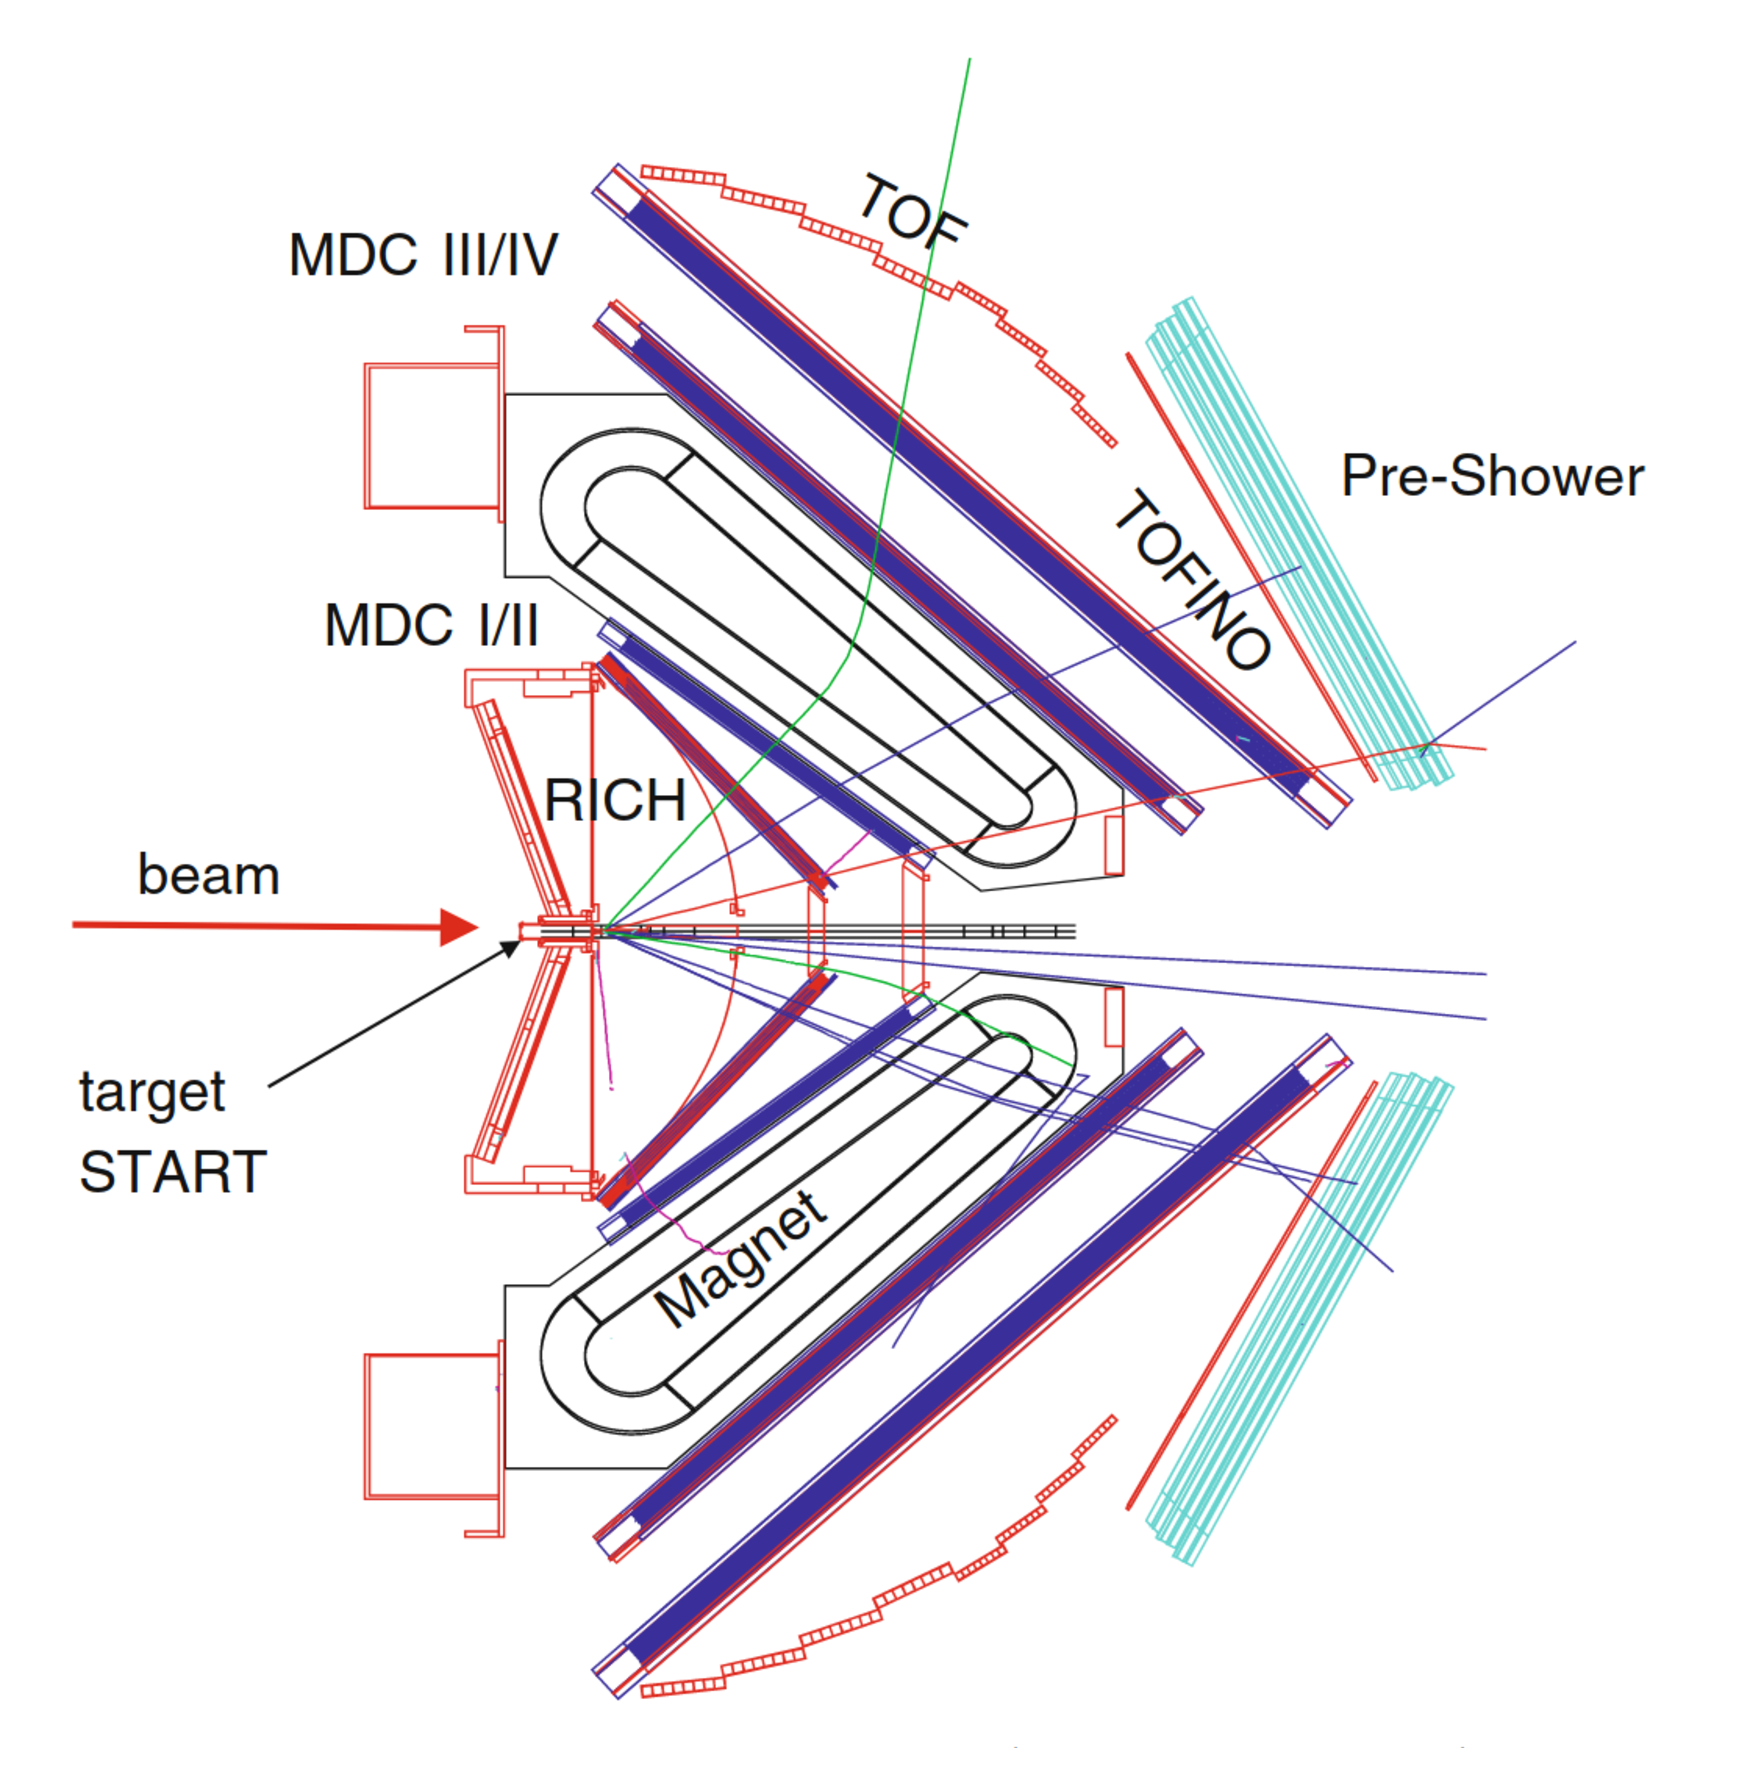
\includegraphics[width=0.7 \linewidth]{Chapter_detector/detektor.eps}
  \caption{The HADES - \cs through the detector. All essential sub-systems used during pp and pNb experiment are visible in the picture. The picture from \cite{Agakishiev:2009am}.}
\end{figure}


\section{Tracking system}
The HADES tracking system bases on four sets of a drift chambers. Two before, and two after a magnetic field. The first set is called inner MDC, the second outer MDC. Each single drift chamber has a trapezoidal shape and consist of 13 layers of wires. They create 6 layers of a drift cells. A shape of the sells and the wires density was optimized to get the best momentum resolutions.

In between inner- and outer-MDC the \textbf{I}ron\textbf{L}ess \textbf{S}uperconducting Electron (ILSE) Magnet is located. It consist of six superconducting coils, which produce a toroidal magnetic field of 3.6 T inside the coils. Outside the coils there is no magnetic field, what makes track reconstruction much easier. The operational varys from 0 to 3500 A. 

The magnetic field produced by ILSE bends particles' tracks what allows for a momentum reconstruction. Tracks reconstructed in inner- and outer-MDCs have to be matched together. A dedicated algorithm for this purpose was developed by HADES collaboration and uses solutions of an equation of motion obtained by Runge-Kutta method.

\section{PreShower and META detectors}
During a pp@3.5~GeV and pNb@3.5~GeV experiments the HADEs culminated with a META (\textbf{M}ultiplicity \textbf{E}lectron \textbf{T}rigger \textbf{A}rray) detector. The META system played two main roles: provided en information about particles time of flight and was utilized as a source for a multiplicity trigger. The detector consisted of two sub-systems: a TOF for polar angles from 44 to 88 degrees and a TOFino angles from 18-45 degree. They also differed by a time resolution $\sigma_{TOF}\approx~150~\mathrm{ps}$, $\sigma_{TOFino}\approx~450~\mathrm{ps}$. The main difference between these detectors was in space resolution properties. Each strap of the TOF detector has a readout at both ends of scintilator. It allows for an estimation of an interaction place base on a time difference between signal arrival in both ends of the detector. Due to economical circumstances the TOFino detector has much smaller granulation and a reed out was installed at one end of each strap. It caused much worse space resolution for the TOFino than for the TOF detector.

An information about interaction point for TOFino detector is given by PreShower detector, located behind the TOFino. Its main purpose was to enhance a capability for lepton identification for polar angles below 45$\deg$. In principle it was a thin, three layer, electromagnetic calorimeter, although it didn't take a role of an energy measurement. It was too thin to fully stop leptons, but thick enough to observe a beginning of an electromagnetic cascade. The detector consisted of three drift chambers layered with two led plates and an energy deposited in each drift chamber was registered. In case of leptons total charge collected for 2nd and 3rd are higher than for 1st. For hadrons deposited energy does not change with detector layer. The detector was used for both: leptons identification and lepton trigger (LVL2).

\section{RICH detector}
The \textbf{R}ing \textbf{I}maging \textbf{CH}erenkov detector is the main tool for $\epem$ identification for the HADES. It is designed  for leptons with momentum between 15 MeV/c and 1.5 GeV/c The detector active area surrounds target area and it is filled by a radiator gas ($\mathrm{C}_4 \mathrm{F}_{10}$). A refractive index gives a threshold speed for a Cherenkov radiation production $\gamma_{thr} =18$. For projectile energies delivered by the SIS18 synhrotron the only particles able to exceed the threshold are electrons end positrons. Passing across the radiator they produce a cone of a Cherenkov light. Then, the light is reflected by a spherical mirror and detected by a pad plane located upstream a beam. An special algorithm called ''\textbf{R}ing \textbf{F}inder'' \cite{hades_RICH} reconstructs Cherenkov light rings from a pattern of fired pads. A reconstructed ring position is matched with track from MDC to assign information about a leptonic character to proper track.  The detector is completely ''hadron blind'' what means that no hadron can give an signal in it. In 2019 the RICH was updated by a new readout system, described more detailed in next section.

The RF algorithm bases on a ring-shape mask. Thanks to very low electron mass, the same velocity for all leptons can be assumed, what causes constant length of a cherenkov rings' diameter. The mask is compared with a pattern registered by pad plain for every event. In case of positive match, a track direction, measured in RICH is compared with all tracks measured in MDC. A fit window between parameters measured in MDC and in RICH is a free parameter and has to be adjusted by user, depending on an expected purity of a leptonic sample.
\begin{figure}
  \centering
  \includegraphics[width=0.6 \linewidth]{Chapter_detector/RICH.png}
  \caption{The \cs of the RICH detector.}
\end{figure}

\section{Target system}
The HADES detector allows for experiments with many different collision systems, starting from pp ending at heavy ion collisions. That versatility is followed by many challenges in a target construction. The target has to be adjusted for specific beam requirements. For this thesis two different systems were investigated pp@3.5 GeV and pNb@3.5 GeV.

\subsection{Target for pp@3.5 GeV}
During the experiment a liquid hydrogen (LH2) target was used. The hydrogen was stored in a special tank designated to keep constant temperature 20K (fig. \ref{fig:target}). Its length was 50 mm, what corresponds to interaction probability 0.7\% for protons with kinetic energy 3.5 GeV. The beam density reached $10^6$ particles/s. For data selection a two-level trigger was used. The first level trigger (LVL1) was dedicated to hadronic reactions and required at least three charged particles registered in META detectors. More over, to reduce a data flux only every third LVL1 event was recorded by DAQ system and stored for further analysis. During four-weeks experimental campaign in total $1.14 \times 10^9$ LVL1 events were recorded \cite{hades_inclL_35}. The second level (LVL2) was dedicated for di-lepton studies and bases on combined information from many detectors. The trigger system search di-lepton pairs bases on information from: RICH detector (Cherenkov light rings), TOF detectors ($\beta>??$) and pre-shower detector (electromagnetic cascade)\cite{Agakishiev:2009am,hades_DAQ}. In case of any signature of a leptonic nature of the tracks they are saved without any down-scaling.

\begin{figure}[ht]
  \centering{}
  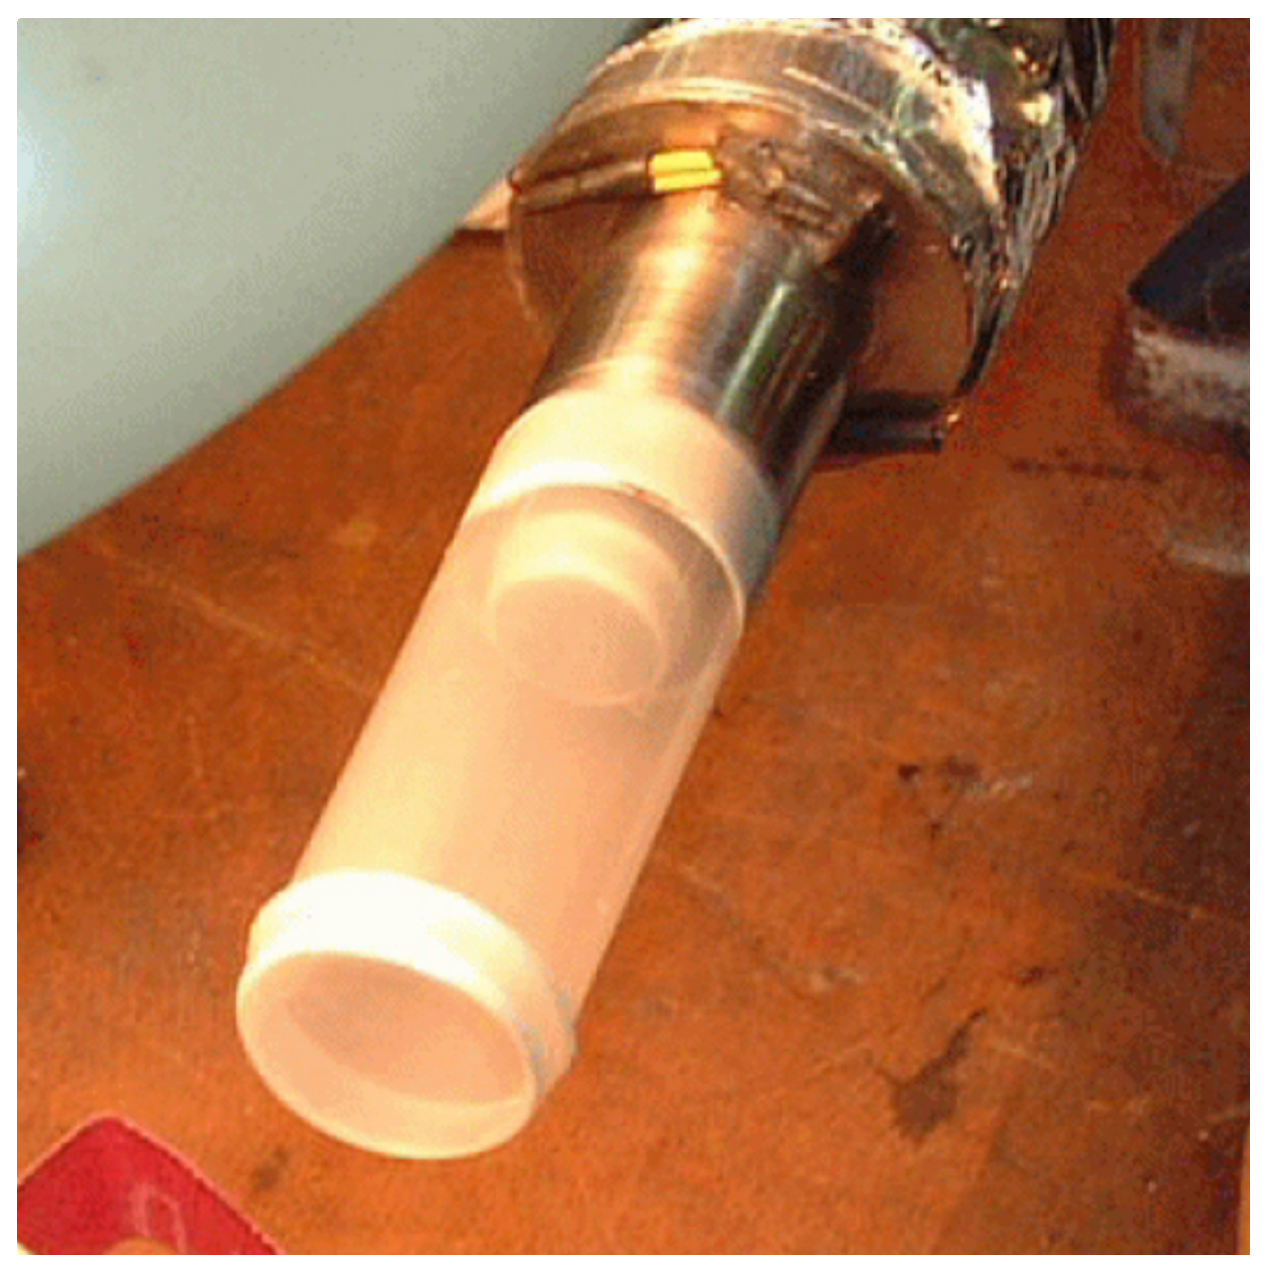
\includegraphics[width=0.7 \linewidth]{Chapter_analysis/tarcza.eps}
  \caption{The LH$_2$ container used during the pp @3.5 GeV experiment.}
  \label{fig:target}
\end{figure}

Due to technical circumstances the pp experiment was conducted without the start detector. A time of flight for each particle was calculated based on a difference between different particles time of flight related to arbitrary experiment clock. Details of the reconstruction method are described in \cite{dybczak_phd}. However in following studies an information from TOF detectors was not required at all, so that information played only secondary role and helped cross-check a de/dx identification method.

\subsection{Target for pNb@3.5 GeV}
The p(3.5 GeV)+Nb experiment was conducted in October 2008. The beam with kinetic energy 3.5 GeV was delivered by the SIS 18 synchrotron and aimed into a segmented, 12-fold target. Each target element had a diameter equal 1.25 mm and 0.45 mm of a thickness. The target parameters were adjusted to get a 2.8\% interaction probability. The trigger system was the same as for pp@3.5 GeV experiment with LVL1 trigger based on hits multiplicity in META detector and LVL2 trigger dedicated for di-lepton studies. During experiment an avrege beam intensity was $2 \times 10^6$ particles/s, what gave in total $3.2 \times 10^9$ LVL1 events recorded on tapes.  

\begin{figure}[ht]
  \centering
  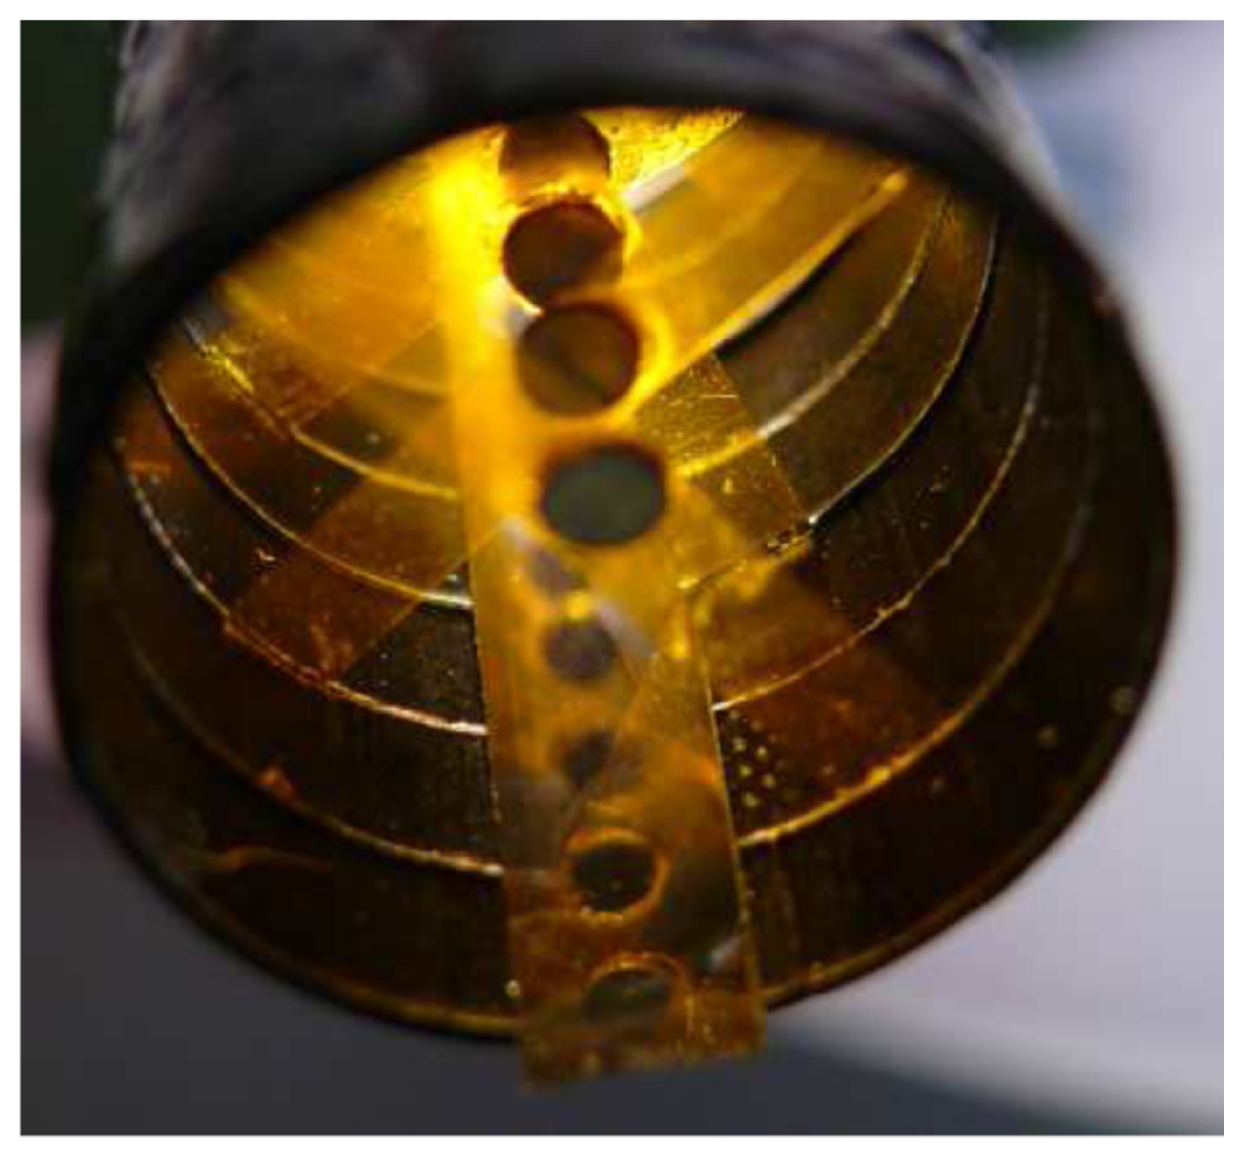
\includegraphics[width=0.7 \linewidth]{Chapter_analysisPNb/target_pNb.eps}
  \caption{The segmented niobium target used for an experiment. Niobium roundels are mounted by a tape inside a carbon tube.}
\end{figure}



\section{The HADES upgrades}
\label{chapter:HADES_upgrades}
Currently HADES is intensively upgraded to face a new physical program. A brand new \textbf{E}lectromagnetic \textbf{CAL}orimeter \cite{FAIRness:Hudoba,FAIRness:Shabanov} and a new RICH readout system have been already installed and tested during campaign with Ag+Ag collisions. In addition a new \textbf{F}or\textbf{W}ard \textbf{DET}ector \cite{FAIRness:Malige} was installed in 2020. It will extend the HADES acceptance to very forward angles, between~$0.6^{\circ}$~and~$7^{\circ}$. One of the main reasons for FwDet development are hyperon studies. This detector will significantly enhance the acceptance for $\Lz$ reconstruction, since momentum conservation causes the proton from $\Lambda$ decay tend to be emitted at small polar angles.Detail about new possibilities for hyperon research opened by the FwDet are presented in. \ref{chapter:simulations}.
\begin{figure}[ht]
  \centering
  \includegraphics[width=0.6 \linewidth]{Chapter_detector/HADES.png}
  \caption{The HADES detector with new updates. Parts labeled by a red font have been installed in 2019 or later and are discussed in following subsection.}
\end{figure}
\subsection{The Forward Detector}
\label{subsec:FwDet}
In many studies, especially devoted to hyperons' decays the forward angles play very important role. The HADES detector for a quite long time did not have a possibility to register particles emitted into polar angle below 10 degree. That situation is changing because of a new \textbf{F}or\textbf{w}ard~\textbf{Det}ector build in a collaboration between Jagiellonian University Cracow, Institut de Physique Nucléaire d'Orsay and Forschungszentrum Jülich.

\begin{figure}[hb]
  \centering
  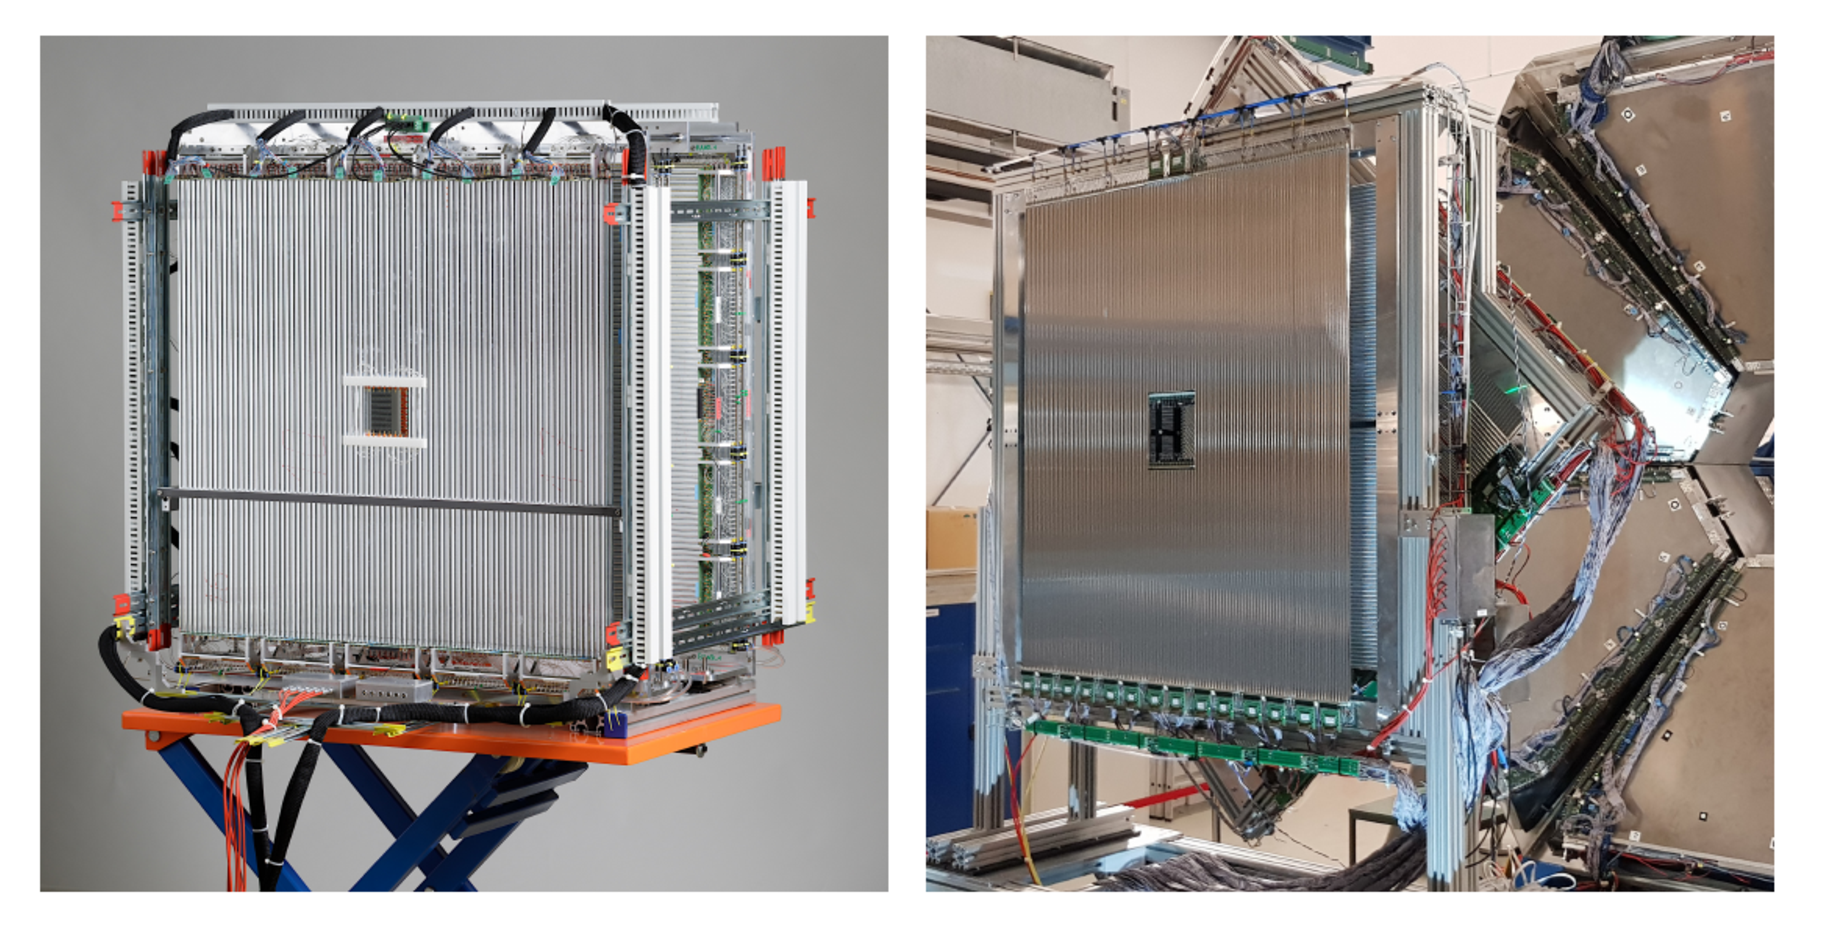
\includegraphics[width=0.6 \linewidth]{Chapter_detector/FwDet.eps}
  \caption{Both tracking stations of the FwDet detector, left: STS1, right: STS2}
\end{figure}

FwDet is a tracking detector consist of two tracking stations: STS1 and STS2. They are made utilizing the same technology as planned forward detector for the PANDA experiment. Each of the stations consist of a set of straws filled by a ArCO$_2$ gas under a pressure of 2 bar. Straws are collected end glued together in modules, 32 straws each. Such a structure, together with overpresure, makes the detector self-supporting. The operational voltage between an anode wire, which is located in center of each straw, and cathode a straw is 1800 V. It resulting a gas gain $5 \cdot 10^4$ and maximum drift time 130 ns. The spatial resolution for single straw is 0.13 mm [ref].

In the STS1 straws are organized in four double-layers aligned by an inclination $0\deg, 90\deg, 0\deg, 90\deg$. The STS2 also consist of four layers but, for better tracking abilities two of them are twisted by $45\deg$. A similar solution was not possible for the STS1 because of lack of a space in ECAL create. The STS2 ends by an RPC detector which provides a precise information about time-of-flight for each track.

Besides a hardware development, track reconstruction and tracking algorithms were developed in Jagiellonian University. A track reconstruction bases on an assumption that between the stations there is no magnetic field. It meas that all tracks are straight lines, and only kinematic variable is a time of flight measured by RPC. It means that it is impossible to make an unambiguous identification of detected particles and some kind of information have to be assumed. The reconstruction procedure using FwDet is described more detailed in \ref{chapter:simulation_identyfication}. Details of the detector structure and prepared software are described in [artykul Rafala]. 
\subsection{RICH update}

\subsection{Electromagnetic calorimeter}
In 2018 first four sector of a new \textbf{E}lectromagnetic \textbf{CAL}orimeter was commissioned. In final stage the ECAL is going to consist of six toroidal sectors, that reflect a general HADES symmetry. They will be assembled at the end of the detector and will replace pre-shower detector. In final configuration, with all six sectors the calorimeter will have almost full azimuntal covering and 12 to 45 degree covering in polar angle. Its main purpose is to extend the HADES capabilities by a photon detection - a capability complementary to di-lepton reconstruction provided by RICH. It will allow for a reconstruction of a neutral mesons and barionic resonances' photo-decays.

\begin{figure}[ht]
  \centering
  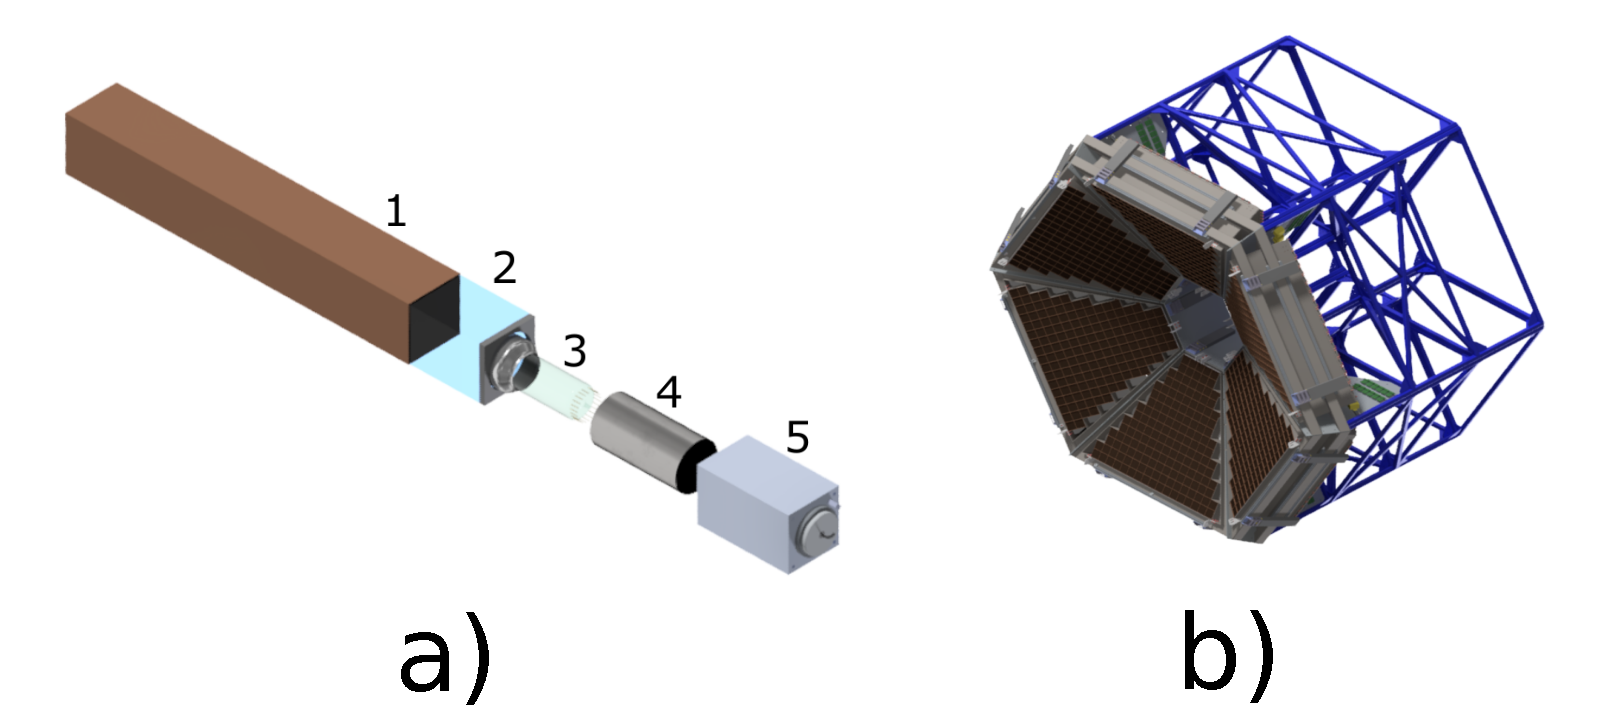
\includegraphics[width=0.9 \linewidth]{Chapter_detector/ECAL.eps}
  \caption{The ECAL detector: a) single module, b) entire apparatus. Each module consists of following parts: 1-brass envelope, 2-lead-glass radiator, 3-photomultiplayer, 4-magnetic shielding, 5-aluminium housing for PMT. The figure from \cite{FAIRness:Hudoba}.}
\end{figure}


The calorimeter consist of 163 modules, each of them composed of a brass envelope a lead-glass prism and a photomultiplayer enclosed in MUMETALL shielding. A high energy photon propagating through a glass causes an electromagnetic cascade. Charged particles from the cascade, mostly $\epem$ pairs, traveling across the led-glass produce a cherenkov light. Next, cherenkov-light photons are detected by a photomultiplayer at the end of the module. Designed resolution, verified by experiment, is $\frac{\Delta E}{E}=5.5\%$ for 1 GeV photons.


